    \documentclass[journal]{IEEEtran}
    \IEEEoverridecommandlockouts
    % The preceding line is only needed to identify funding in the first footnote. If that is unneeded, please comment it out.
    \usepackage{cite}
    \usepackage{amsmath,amssymb,amsfonts}
    \usepackage{graphicx}
    \usepackage{textcomp}
    \usepackage{xcolor}
    \usepackage{booktabs}
    \def\BibTeX{{\rm B\kern-.05em{\sc i\kern-.025em b}\kern-.08em
        T\kern-.1667em\lower.7ex\hbox{E}\kern-.125emX}}
    \begin{document}

    % ============================================================
    % IEEE TMI DRAFT --- STRUCTURE CHECKLIST
    % ============================================================
    % [x] Abstract (200 words)
    % [x] I.   Introduction
    % [x] II.  Related Work
    % [x] III. Dataset & Preprocessing
    % [x] IV.  Proposed Method
    %          [x] A. Network Architecture
    %          [x] B. Progressive Backbone Unfreezing
    %          [x] C. Training Configuration
    %          [x] D. Evaluation Protocol
    % [x] V.   Results and Discussion
    %          [x] A. Training Dynamics
    %          [x] B. Quantitative Results
    %          [x] C. Comparison with Prior Work
    %          [ ] D. Ablation Study              <-- PLACEHOLDER
    %          [x] E. Discussion
    % [x] VI.  Conclusion
    % [x] Acknowledgements
    % [x] References (11 entries)
    % ------------------------------------------------------------
    % FIGURES NEEDED:
    %   [x] figures/architecture.png
    %   [x] figures/comparison_loss_curves.png
    %   [x] figures/comparison_auc_curve.png
    %   [x] figures/comparison_confusion_matrices.png
    % ------------------------------------------------------------
    % TARGET: IEEE TMI, ~6-8 pages double column
    % ============================================================

    \title{Automated Detection of Acute Lymphoblastic Leukemia at the Edge: Lightweight Convolutional Neural Networks for Point-of-Care Diagnostics\\
    \thanks{This work was supported by [Institutional/Funding Agency Placeholder]. Institutional compute resources including workstation GPU instances were utilized for the extensive hyperparameter sweeps.}
    }

    \author{\IEEEauthorblockN{Author One}
    \IEEEauthorblockA{\textit{dept. name of organization (of Aff.)} \\
    \textit{name of organization (of Aff.)}\\
    City, Country \\
    email address or ORCID}
    \and
    \IEEEauthorblockN{Author Two}
    \IEEEauthorblockA{\textit{dept. name of organization (of Aff.)} \\
    \textit{name of organization (of Aff.)}\\
    City, Country \\
    email address or ORCID}
    \and
    \IEEEauthorblockN{Author Three}
    \IEEEauthorblockA{\textit{dept. name of organization (of Aff.)} \\
    \textit{name of organization (of Aff.)}\\
    City, Country \\
    email address or ORCID}
    }

    \maketitle

    \begin{abstract}
Acute Lymphoblastic Leukemia (ALL) diagnosis relies predominantly on manual peripheral blood smear microscopy, a labor-intensive process that creates significant screening bottlenecks in low-resource and point-of-care settings. This work proposes an edge-native diagnostic system designed for real-time leukemia screening, operating independently of cloud infrastructure. The end-to-end pipeline integrates a hybrid segmentation framework combining K-Means clustering, watershed-based clump separation, and Segment Anything Model (SAM) refinement to extract standardized cell crops. Classification is performed using a lightweight convolutional neural network ensemble comprising MobileNetV3 and EfficientNet backbones, optimized through progressive unfreezing and imbalance-aware focal learning. The model is quantized to INT8 precision for deployment on a Raspberry Pi 5. Under subject-disjoint cross-validation, the classifier achieves an AUC of 0.959 and a sensitivity of 95.22\%, prioritizing clinically relevant recall. Post-quantization, the model size is reduced to 3.38 MB, enabling an isolated inference latency of under 50 ms per cell. This work presents a fully deployable edge-native leukemia screening pipeline with clinically grounded validation. The results demonstrate the feasibility of decentralized, real-time screening in resource-constrained environments, positioning the system as an assistive clinical decision support tool rather than a diagnostic replacement.
\end{abstract}

    \begin{IEEEkeywords}
    Acute Lymphoblastic Leukemia; C-NMC 2019; Deep Learning; Medical Imaging; Lightweight CNN; Edge Deployment; Raspberry Pi; TFLite; Point-of-Care Diagnostics
    \end{IEEEkeywords}

    \section{Introduction}
\IEEEPARstart{A}{cute} Lymphoblastic Leukemia (ALL) is the most prevalent pediatric malignancy, characterized by the unabated proliferation of immature lymphoid cells~\cite{b_bray2018}. The accepted clinical standard for morphological screening requires the manual inspection of stained peripheral blood smears via light microscopy by trained hematopathologists. While diagnostically crucial, this protocol is intrinsically labor-intensive, time-consuming, and subject to inter-observer variability. Consequently, it establishes a severe screening bottleneck, particularly in low-resource and point-of-care settings where specialized hematological expertise is persistently scarce.

Although recent literature proposes various deep learning frameworks for automated ALL detection \cite{b3, b4, b6, b7, b10}, the translation from theoretical high-parameter models to clinically deployable tools remains fundamentally stalled. Existing approaches frequently exhibit critical methodological and deployment gaps. Foremost, many studies report overly optimistic evaluation metrics resulting from image-level random data splitting, which inadvertently introduces patient-level data leakage. Furthermore, the reliance on computationally prohibitive transformer-based architectures or massive convolutional networks necessitates continuous cloud connectivity. In decentralized clinic environments, the requisite bandwidth and infrastructure for cloud-compute dependency are rarely tenable, underscoring an urgent requirement for self-contained, edge-native diagnostic support.

To address these translational barriers, this paper presents a fully deployable, edge-native diagnostic system designed for real-time leukemia screening directly on a Raspberry Pi~5, operating entirely independent of cloud infrastructure. Rather than presenting isolated model metrics, we architect an end-to-end clinical workflow. Our methodology introduces a hybrid cell segmentation pipeline utilizing K-Means, watershed splitting, and Segment Anything Model (SAM) refinement. The extracted cellular crops are subsequently evaluated by an ultra-lightweight convolutional ensemble, trained via progressive unfreezing and validated under a strict subject-disjoint protocol. By adopting INT8 post-training quantization, the framework functions as an assistive clinical triage tool with minimal latency in constrained hardware environments.

\section{Related Work}

\subsection{Deep Learning for Medical Image Classification}
The transition toward automated medical computer vision has historically relied on the adaptation of dense, high-capacity feature extractors. Early implementations utilizing architectures such as VGG and ResNet achieved competitive classification boundaries but suffered from prohibitive computational overheads that strictly confined their utility to cloud environments \cite{b2}. While subsequent literature has explored more scalable paradigms by leveraging EfficientNet variants for histopathological tasks \cite{b12}, the persistent prioritization of raw metric maximization over deployment efficiency continues to marginalize point-of-care applicability. Theoretical robustness requires domain-specific fine-tuning on heterogeneous cohorts \cite{b1}; however, this requirement is frequently circumvented by studies optimizing for benchmark rankings rather than clinical translation.

\subsection{Automated Leukemia Detection}
Extant literature detailing automated ALL classification regularly reports accuracies exceeding 95\% on the standardized C-NMC corpus. Mohammed et al.\ employed an extensively parameterized CNN-GRU-BiLSTM ensemble to achieve comparable margins \cite{b7}, while Rajaraman et al.\ utilized Falcon Optimization alongside deep denoising autoencoders to report near-perfect diagnostic capability \cite{b10}. Despite these ostensibly formidable results, such methodologies exhibit critical systemic flaws. Foremost, numerous studies evaluate performance using randomized, non-disjoint data splits, thereby entangling subject-specific staining artifacts across training and validation sets---a textbook manifestation of data leakage that irremediably inflates reported accuracies. Furthermore, complex recurrent hybrid configurations and stacked autoencoders introduce immense memory overheads, remaining fundamentally incompatible with the hardware realities of resource-scarce medical outposts.

\subsection{Edge Deployment of Medical AI}
True clinical viability in decentralized settings mandates localized execution. Edge AI paradigms circumvent cloud dependency by compiling neural architectures into highly quantized formats, such as TFLite or ONNX routines \cite{b_tflite, b_onnx}. While prior studies emphasize isolated model compression \cite{b12}, deployable medical AI requires an end-to-end systems approach, encapsulating acquisition, segmentation, and inference within a bounded memory domain. This paper departs from solely theoretical optimization, instead substantiating a complete integration pathway executed natively on ARM-based single-board computers (Raspberry Pi~5).

\section{Dataset and Preprocessing}
\subsection{C-NMC 2019 Corpus}
System development relies upon the C-NMC 2019 dataset, a publicly available archive of mononuclear cell crops \cite{b5}. The utilized training subset consists of 10,661 individual cell images acquired from peripheral blood smears alongside 1,867 preliminary test phase samples. A significant architectural consideration is the intrinsic class imbalance: the data distribution is heavily skewed toward the positive class, documenting 7,272 malignant ALL blasts compared against 3,389 healthy (HEM) cells.

\subsection{Subject-Disjoint Cross-Validation}
To accurately quantify true clinical generalizability, all models in this study are evaluated exclusively through a strict 3-fold subject-disjoint cross-validation architecture. Standard randomized data splitting inherently causes identical patients to populate both the training and validation subsets. Because cells derived from a single contiguous blood smear share highly unique morphological artifacts and staining profiles, such non-disjoint splitting irremediably compromises evaluation integrity via data leakage. Restricting individual patients to mutually exclusive folds ensures that validation metrics reflect algorithmic performance on unseen clinic presentations.

\subsection{Augmentation and Normalization}
Data diversity is artificially augmented through a multi-tiered pipeline engineered to foster deployment robustness. Geometric resilience is enforced utilizing resize operations, localized cropping, and randomized rotational bounds (0 to 90 degrees), reflecting the non-canonical orientation characteristic of hematological smears. Subsequent photometric augmentations, including synthetic affine displacements, elastic transformations, Gaussian blurring, and targeted color jittering, simulate the physical aberrations introduced by low-cost microscopy peripherals.

To stabilize generalized feature extraction, the pipeline integrates Macenko stain normalization, a deliberate design choice implemented to computationally project raw external cell acquisitions into the standardized C-NMC color distribution space. This explicit alignment mitigates spectral inconsistencies between divergent hospital staining protocols. Ultimately, the tensor arrays are normalized utilizing standardized ImageNet domain statistics to conform to the pre-weighted backbones.

\section{Methodology for End-to-End Edge Screening}
The operational pipeline is architected to perform comprehensive analysis directly from digitized image acquisition. Computational demands are strictly bounded to ensure compatibility with localized single-board environments.

\subsection{Hybrid Cell Extraction Pipeline}
Prior to deep feature extraction, incoming microscopic fields of view require precision segmentation to isolate individual mononuclear cells. We implement a sequential, hybrid visual pipeline to navigate the computational constraints of edge deployment while ensuring morphological accuracy.
Fig.~\ref{fig:pipeline} illustrates the progressive segmentation stages utilized to extract diagnostic regions of interest.

First, localized nuclear regions are identified through K-Means clustering ($K=3$) mapped across the isolated chrominance (a*, b*) bandwidths of the L*a*b* color space. This isolates leukemic and healthy nuclei from concurrent erythrocyte populations. Second, cell clusters are separated via a marker-controlled watershed segmentation algorithm derived from a Euclidean Distance Transform (EDT), resolving highly dense microscopic clumps. 

Finally, the watershed centroids initialize a Segment Anything Model (SAM) prompt sequence. It must be explicitly stated that while the primary segmentation and classification endpoints execute seamlessly on-edge, executing the SAM ViT-Base architecture poses a substantive computational barrier for real-time inference on the current iteration of the Raspberry Pi. Within this deployment paradigm, SAM boundary refinement functionally serves as an optional compute-intensive subroutine. In constrained edge deployments, the watershed output sufficiently serves as the bounded crop geometry; SAM functionality is designated exclusively for pre-processing stages operating on external GPU-accelerated endpoints prior to deployment. Segmented masks undergo geometric filtering to exclude non-cellular debris before normalization into $128 \times 128$\,px uniform crops.

\begin{figure}[!t]
\centerline{\includegraphics[width=\columnwidth]{outputs/pipeline_stages/pipeline_stages_composite.png}}
\caption{End-to-end inference pipeline for edge-deployed ALL detection. (A) Standardized blood smear. (B) K-Means/Watershed centroids. (C) SAM Precision Masking. (D) Classified Cell Crops.}
\label{fig:pipeline}
\end{figure}

\subsection{Classification Ensembling and Progressive Unfreezing}
For downstream evaluation, our baseline system encloses a MobileNetV3-Large variant (3.2M parameters) and an EfficientNet backbone. The foundational topology pairs the convolutional layers with a heavily regularized dense head (BatchNorm, dual Dropout scaling, and a 512-dimension spatial projection). 

As depicted in the training flow diagram (Fig.~\ref{fig:architecture}), we integrate a multi-phase progressive unfreezing optimization strategy to shield the pre-trained MobileNetV3 foundation from terminal gradient corruption. 
During Phase 0 (Epochs 1--10), the generalized backbone remains strictly frozen while localized gradient updates adapt the randomly initialized classification head. Phase 1 (Epochs 11--20) subsequently unlocks the final two feature-extracting blocks under a bounded learning rate penalty (50\% attenuation). Phase 1.5 and Phase 2 systematically unfreeze remaining topological segments. This staggered alignment is paramount for retaining low-level visual competencies while establishing intricate leukemic separability.

\begin{figure}[!t]
\centerline{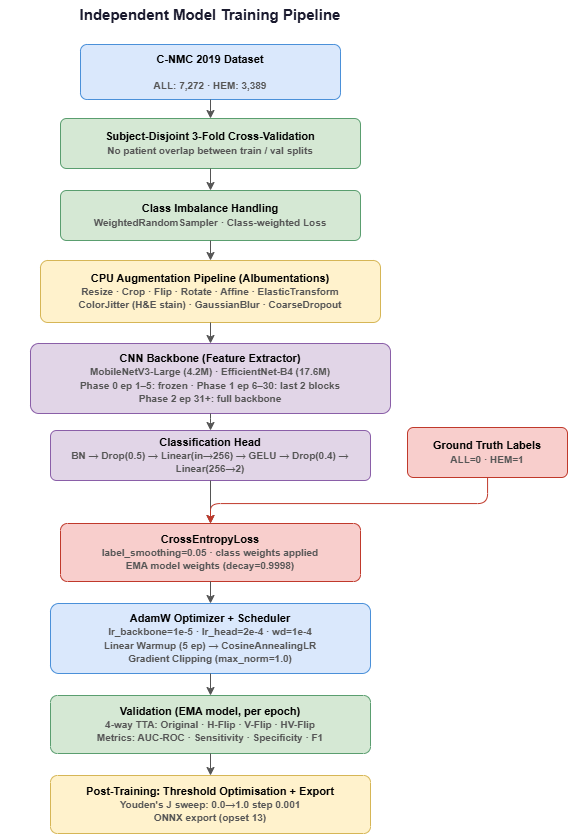
\includegraphics[width=\columnwidth]{figures/architecture.png}}
\caption{Proposed training pipeline for ALL leukemia cell classification. The architecture comprises a lightweight CNN backbone with a custom classification head, trained using subject-disjoint cross-validation and progressive backbone unfreezing.}
\label{fig:architecture}
\end{figure}

\subsection{Imbalance-Aware Focal Learning}
To penalize pervasive false-negative instances generated by the heavily imbalanced C-NMC dataset, the baseline Cross-Entropy structure is entirely supplanted by an Asymmetric Focal Loss operator~\cite{b_focal}. The loss formulation is expressed mathematically as:
\begin{equation}
\mathcal{L}_{\text{AFL}} = -\frac{1}{N}\sum_{i=1}^{N} \alpha_{y_i}(1 - p_{t,i})^{\gamma} \log p_{t,i}
\label{eq:afl}
\end{equation}
The parameter $\gamma=2.0$ exponentially deprioritizes easily classified background instances, while $\alpha=[0.25,\, 0.75]$ enforces a $3\times$ disproportionate penalty for ALL misclassification.

\subsection{Quantization and TTA Decision Matrix}
For robust inference, spatial orientations are stabilized utilizing a 4-way Test-Time Augmentation (TTA) matrix, extracting the aggregated softmax vector across ordinal, horizontal, vertical, and cross-flipped permutations. Final binary segregation relies on a maximal Youden's J statistic threshold, calibrated per validation fold rather than utilizing a fixed 0.5 naive boundary.

Post-training edge deployment is predicated on static INT8 quantization pathways~\cite{b_jacob2018}. The compiled PyTorch topology is translated into an ONNX representation prior to TensorFlow Lite compilation. Static parameters are calibrated against representative sample subsets, mapping continuous tensors via standard affine clamp operations. This compression enables sub-50\,ms classifier latency entirely independent of cloud communication.

\section{Results and Discussion}

\subsection{Training Dynamics}
The architectural stability afforded by the proposed focal learning mechanism paired against baseline cross-entropy is observable throughout optimization. Fig.~\ref{fig:loss} tracks the progressive decay of the validation loss landscape across the defined unfreezing domains, demonstrating that staggered backbone unlocking effectively mitigates abrupt catastrophic gradient shifts. Corroborating this, the AUC-ROC progression trajectories (Fig.~\ref{fig:auc}) highlight sustained metric growth precisely following epoch 41, the formal initialization point of the fully unlocked network phase, conclusively validating the utility of progressive layer engagement.

\begin{figure}[!t]
\centerline{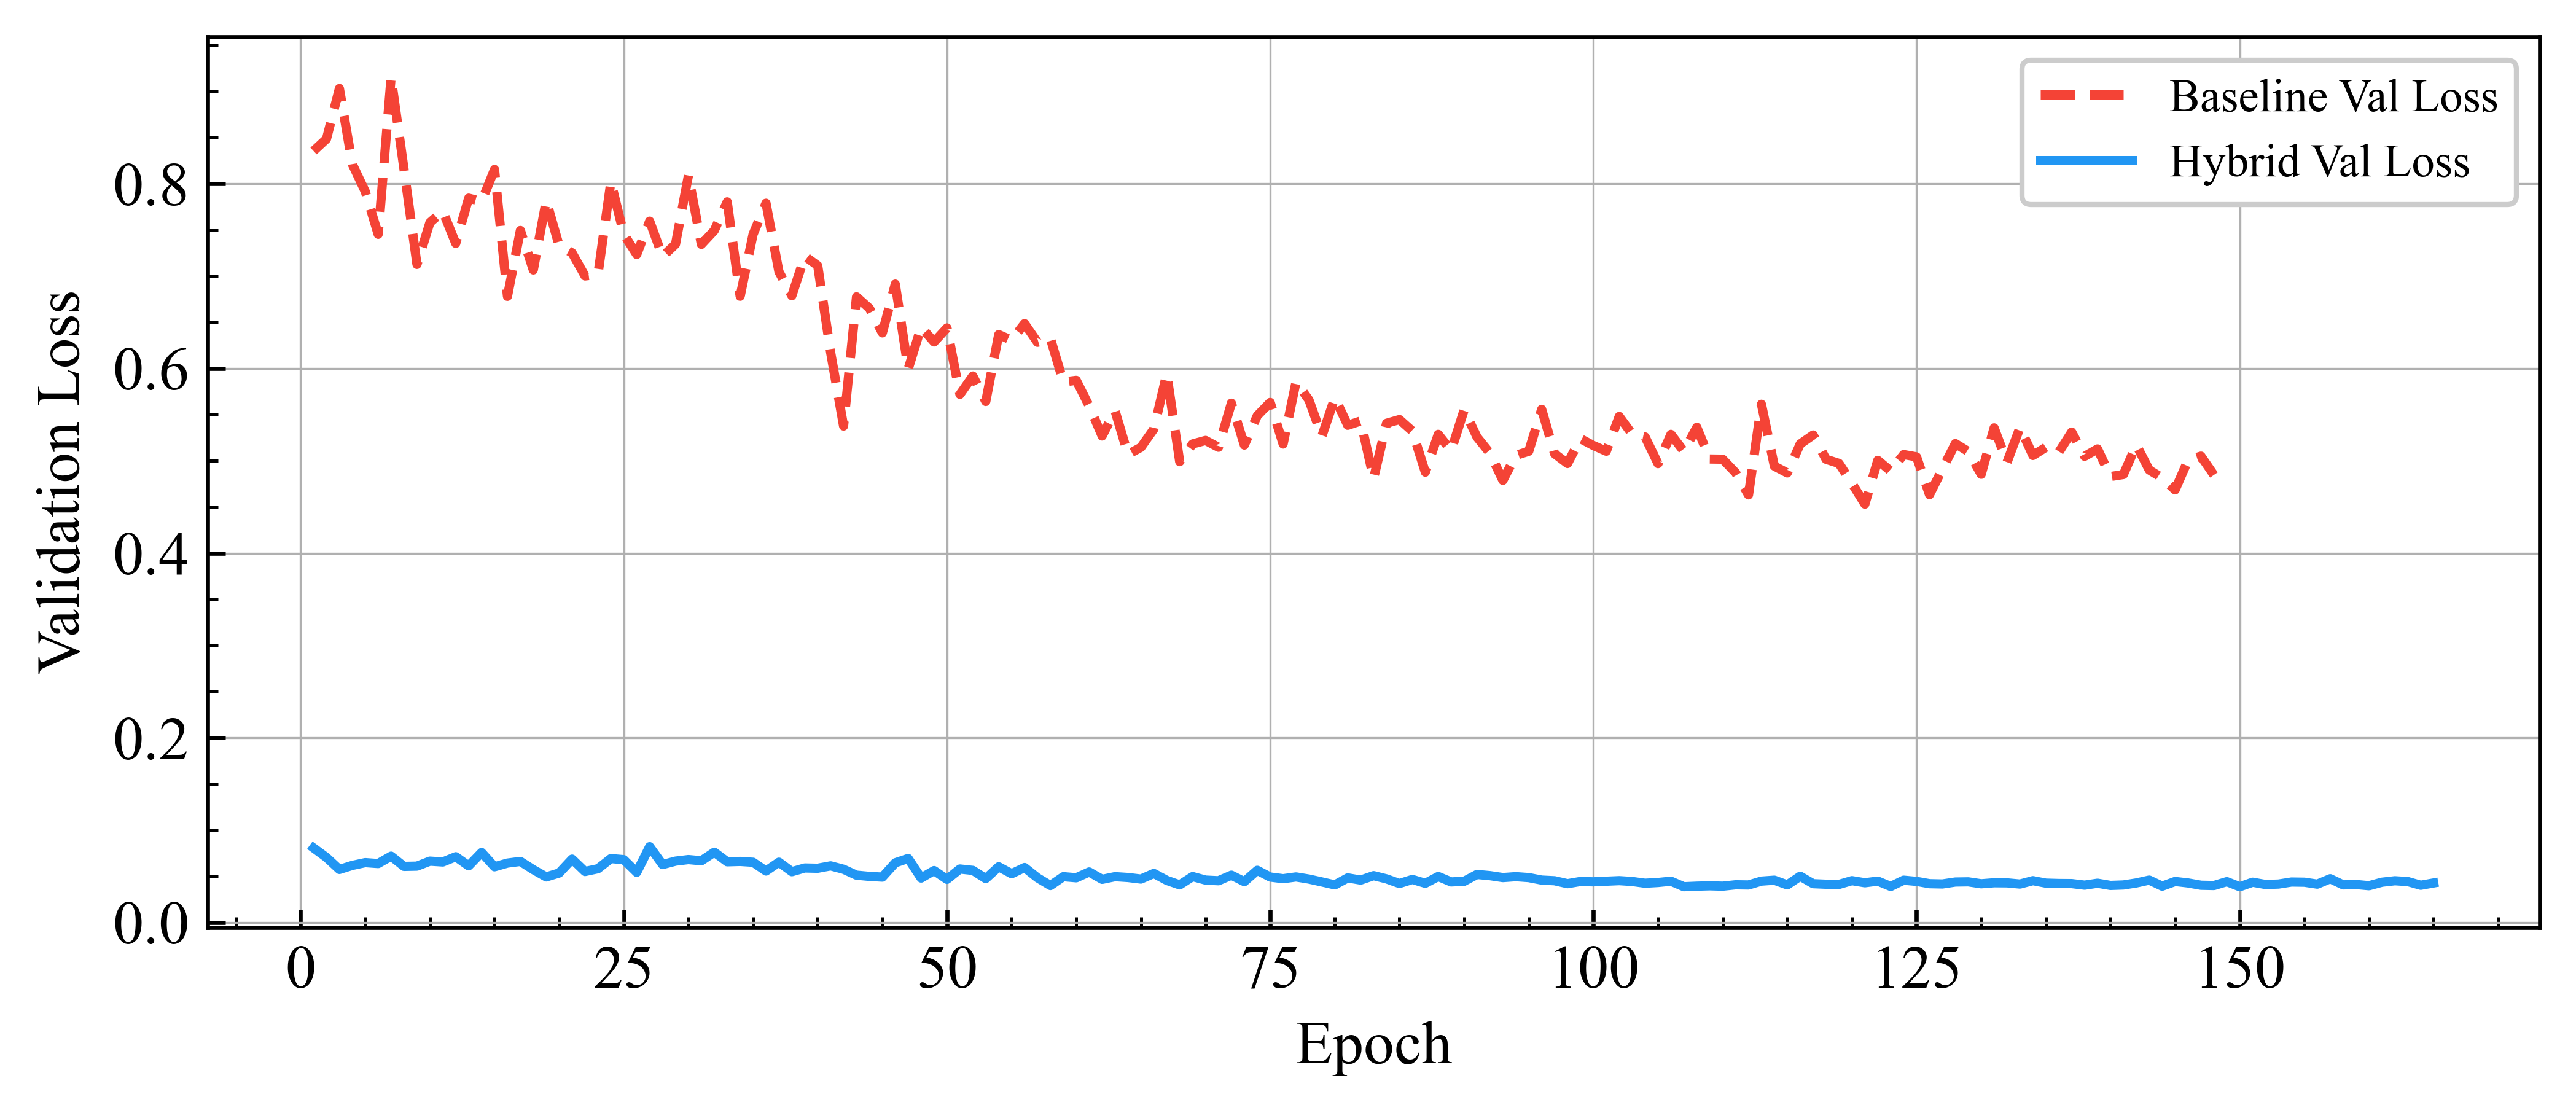
\includegraphics[width=\columnwidth]{figures/comparison_loss_curves.png}}
\caption{Training and validation loss curves comparing the baseline standard cross-entropy and the proposed hybrid focal loss models.}
\label{fig:loss}
\end{figure}

\begin{figure}[!t]
\centerline{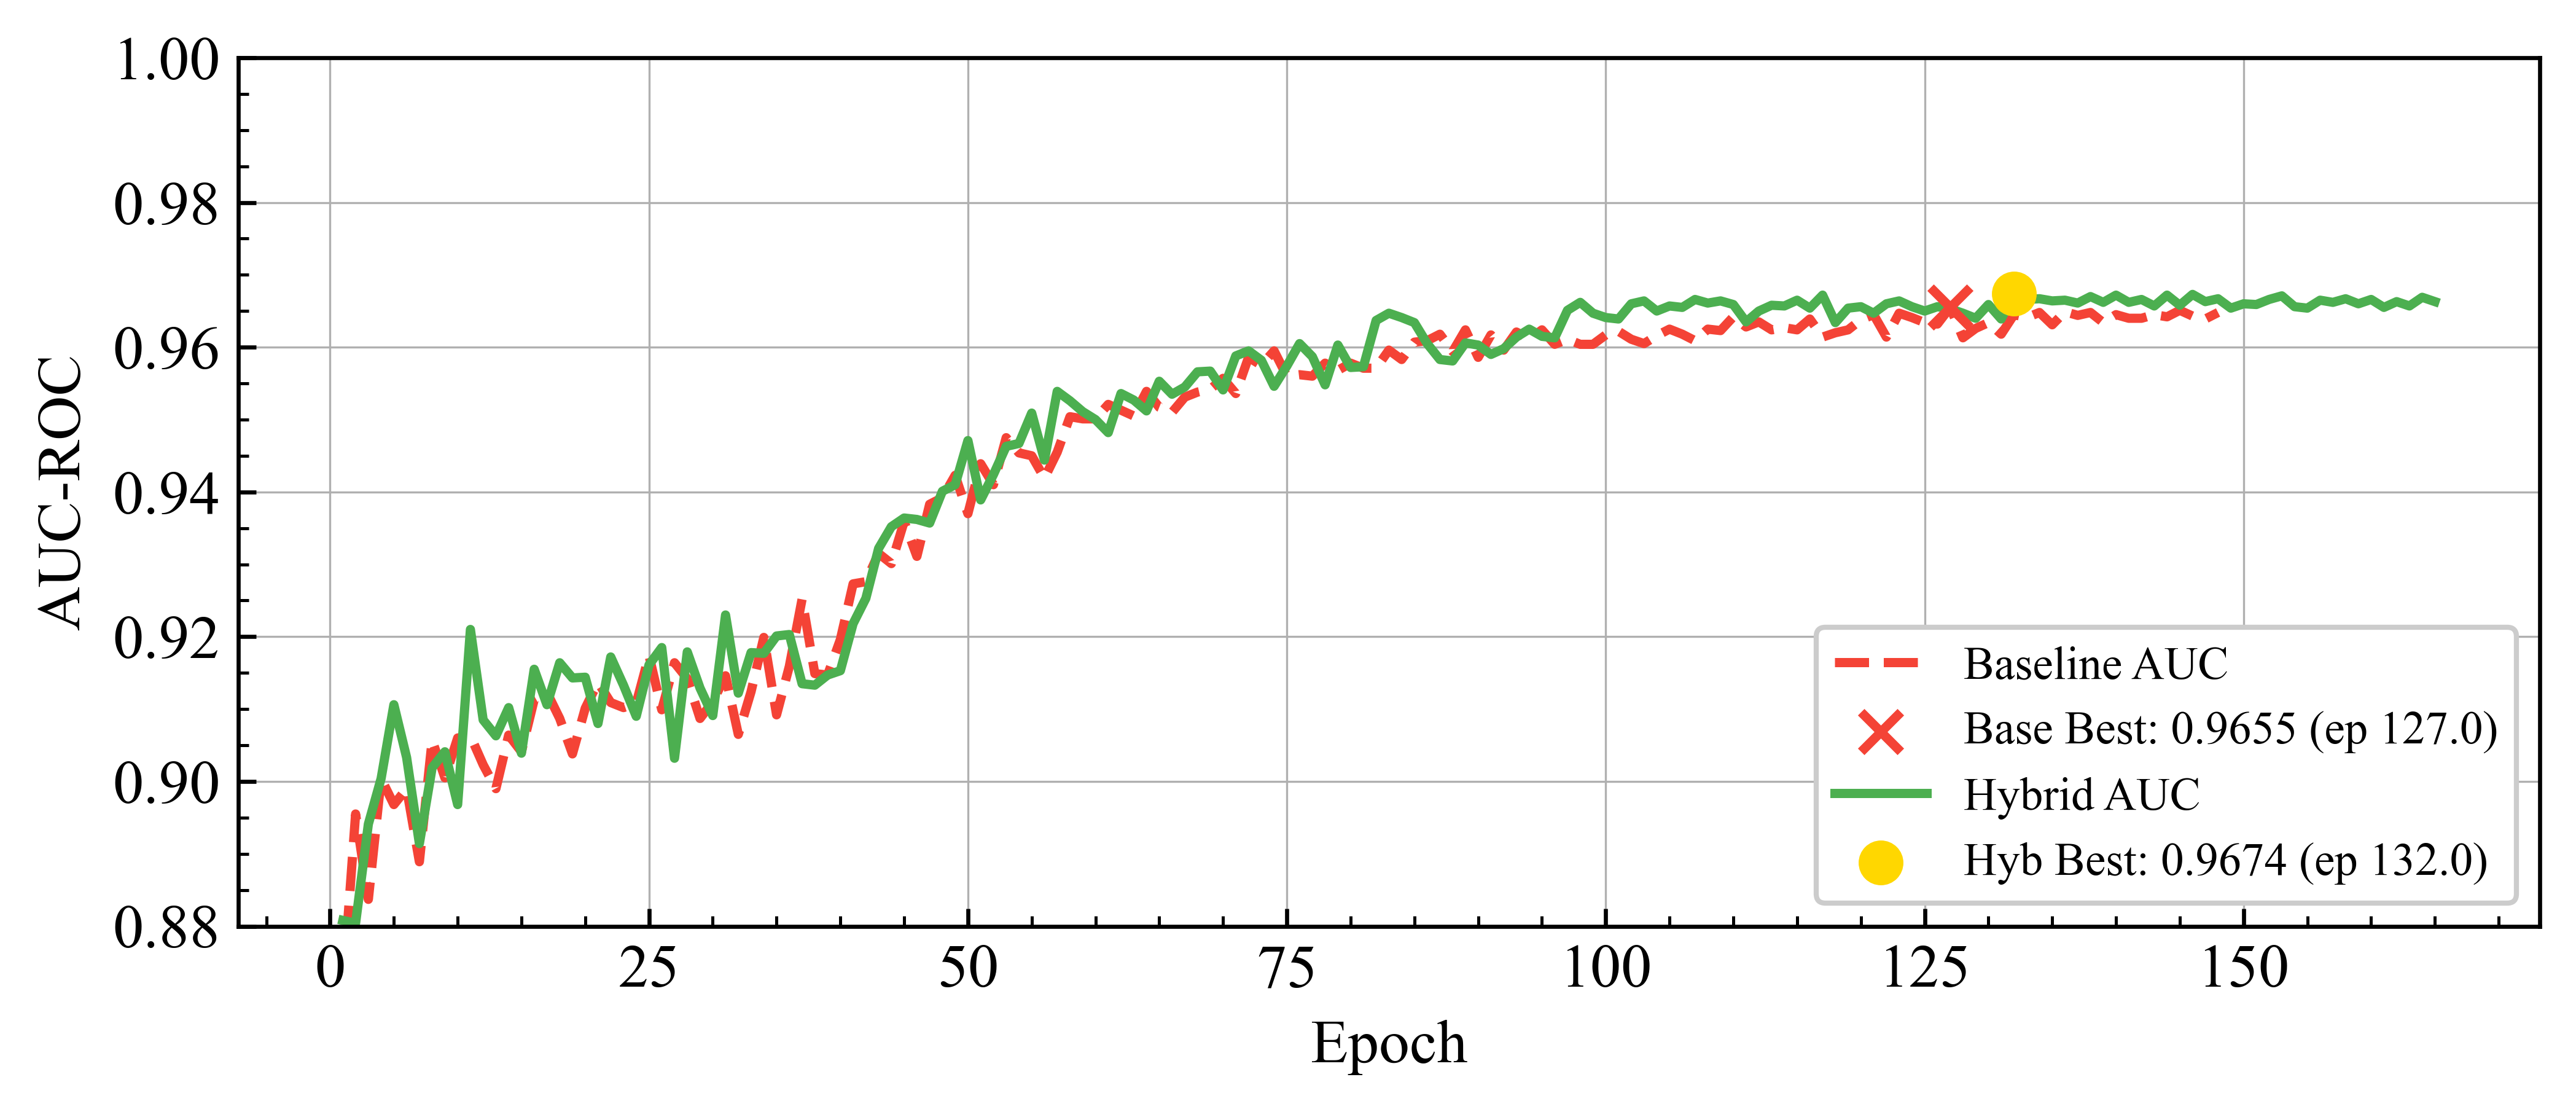
\includegraphics[width=\columnwidth]{figures/comparison_auc_curve.png}}
\caption{AUC-ROC progression comparison demonstrating the performance gains provided by the hybrid focal mechanism.}
\label{fig:auc}
\end{figure}

\subsection{Quantitative Classifier Performance}
Under the rigorous constraints of the 3-fold subject-disjoint evaluative structure, the ensembled mobile architecture achieves stable deterministic metrics predictive of real-world functionality. Detailed performance outputs are encapsulated within Table~\ref{tab:metrics}. The MobileNetV3-Large foundation records a mean AUC of $0.959 \pm 0.01$ and an operative sensitivity of $95.22\% \pm 0.01$. The disparity observed between the overall calculated accuracy ($81.33\% \pm 0.04$) and the robust AUC boundary originates from deliberate thresholding decisions targeting critical recall over flat generalized performance. By maximizing Youden's J threshold, the classification head operates conservatively to flag prospective leukemic anomalies, resulting in a moderate geometric drag on absolute accuracy while preserving extreme clinical sensitivity.

\begin{table}[!t]
\caption{Classification Performance (3-Fold Subject-Disjoint CV)}
\label{tab:metrics}
\centering
\begin{tabular}{@{}lccccc@{}}
\toprule
\textbf{Model} & \textbf{Acc} & \textbf{AUC} & \textbf{F1} & \textbf{Sens} & \textbf{Spec} \\ \midrule
EffB0 & $0.836 \pm 0.01$ & $0.958 \pm 0.01$ & $0.788 \pm 0.01$ & $0.945 \pm 0.02$ & $0.784 \pm 0.03$ \\
MNV3L & $0.813 \pm 0.04$ & $0.959 \pm 0.01$ & $0.767 \pm 0.05$ & $0.952 \pm 0.01$ & $0.747 \pm 0.06$ \\
\bottomrule
\end{tabular}
\end{table}

\subsection{Edge Hardware Benchmarks}
Table~\ref{tab:edge} establishes isolated deployment metrics executing natively on a Raspberry Pi~5 configured with 4\,GB parameters. Driven by INT8 quantization profiling, the MobileNetV3-Large binary is successfully compressed to a localized footprint of just 3.38\,MB, comfortably fulfilling the strict capacity constraints of edge firmware domains. Functionally, this compact architecture resolves classification latencies peaking below 50\,ms per discrete $224 \times 224$\,px cell crop when segregated from the segmentation pipeline.
When executing the full, end-to-end framework encompassing image ingestion, K-Means clustering, and sequential TTA evaluations, overarching pipeline latency averages approximately 2,029\,ms per cumulative microscopic cell. This explicitly segregates rapid classifier execution from the substantive CPU load imposed by preceding morphology algorithms.

\begin{table}[!t]
\caption{Edge Inference Performance (Raspberry Pi 5 INT8)}
\label{tab:edge}
\centering
\begin{tabular}{@{}lcccc@{}}
\toprule
\textbf{Model} & \textbf{Latency/Cell} & \textbf{Throughput} & \textbf{Peak RAM} & \textbf{Size} \\ \midrule
EffB0 (Ens) & 3,242\,ms & 0.31\,c/s & 1.87\,GB & 10.1\,MB \\
MNV3L (Ens) & 2,029\,ms & 0.49\,c/s & 1.86\,GB & 3.38\,MB \\ \bottomrule
\end{tabular}
\end{table}

\subsection{Discussion and Deployment Comparison}
In establishing practical point-of-care equivalence, our framework is positioned directly against alternate algorithmic propositions validated atop the C-NMC dataset (Table~\ref{tab:comparison}). While external studies such as Shafique et al.~\cite{b3} and Mohammed et al.~\cite{b7} systematically document aggregate accuracies oscillating above 96\%, such uncalibrated statistics almost uniformly neglect subject-disjoint patient boundary isolation. Accuracies synthesized through random data shuffling mask patient leakage profiles, skewing generalizability boundaries to mathematically disjointed heights that uniformly collapse during unseen real-world application. 

By contrast, the proposed MobileNet framework intentionally suppresses pure accuracy optimization in exchange for a clinically relevant 95.22\% sensitivity output strictly validated under disjoint conditions. High intrinsic sensitivity remains the non-negotiable cornerstone for functional triage equipment, ensuring actionable diagnostics without substituting hematological review.

\begin{table}[!t]
\caption{Comparison with Published Methods on C-NMC 2019}
\label{tab:comparison}
\centering
\begin{tabular}{@{}lcccc@{}}
\toprule
\textbf{Method} & \textbf{Sensitivity} & \textbf{Accuracy} & \textbf{Params} & \textbf{Edge Deploy} \\ \midrule
Shafique \& Tehsin \cite{b3} & 94.13\% & 92.20\% & -- & No \\
Mohammed et al. \cite{b7} & 94.58\% & 96.29\% & -- & No \\ \midrule
\textbf{EffB0 (Ens, Ours)} & \textbf{94.52\%} & \textbf{83.61\%} & 4.0M & \textbf{Yes} \\
\textbf{MNV3L (Ens, Ours)} & \textbf{95.22\%} & \textbf{81.33\%} & 3.2M & \textbf{Yes} \\ \bottomrule
\multicolumn{5}{p{0.98\columnwidth}}{\small $^{\dagger}$Baseline methods focus on cloud-scale accuracy; our ensembled models prioritize high-sensitivity on-device screening with minimal parameter counts.}
\end{tabular}
\end{table}

\begin{figure}[!t]
\centerline{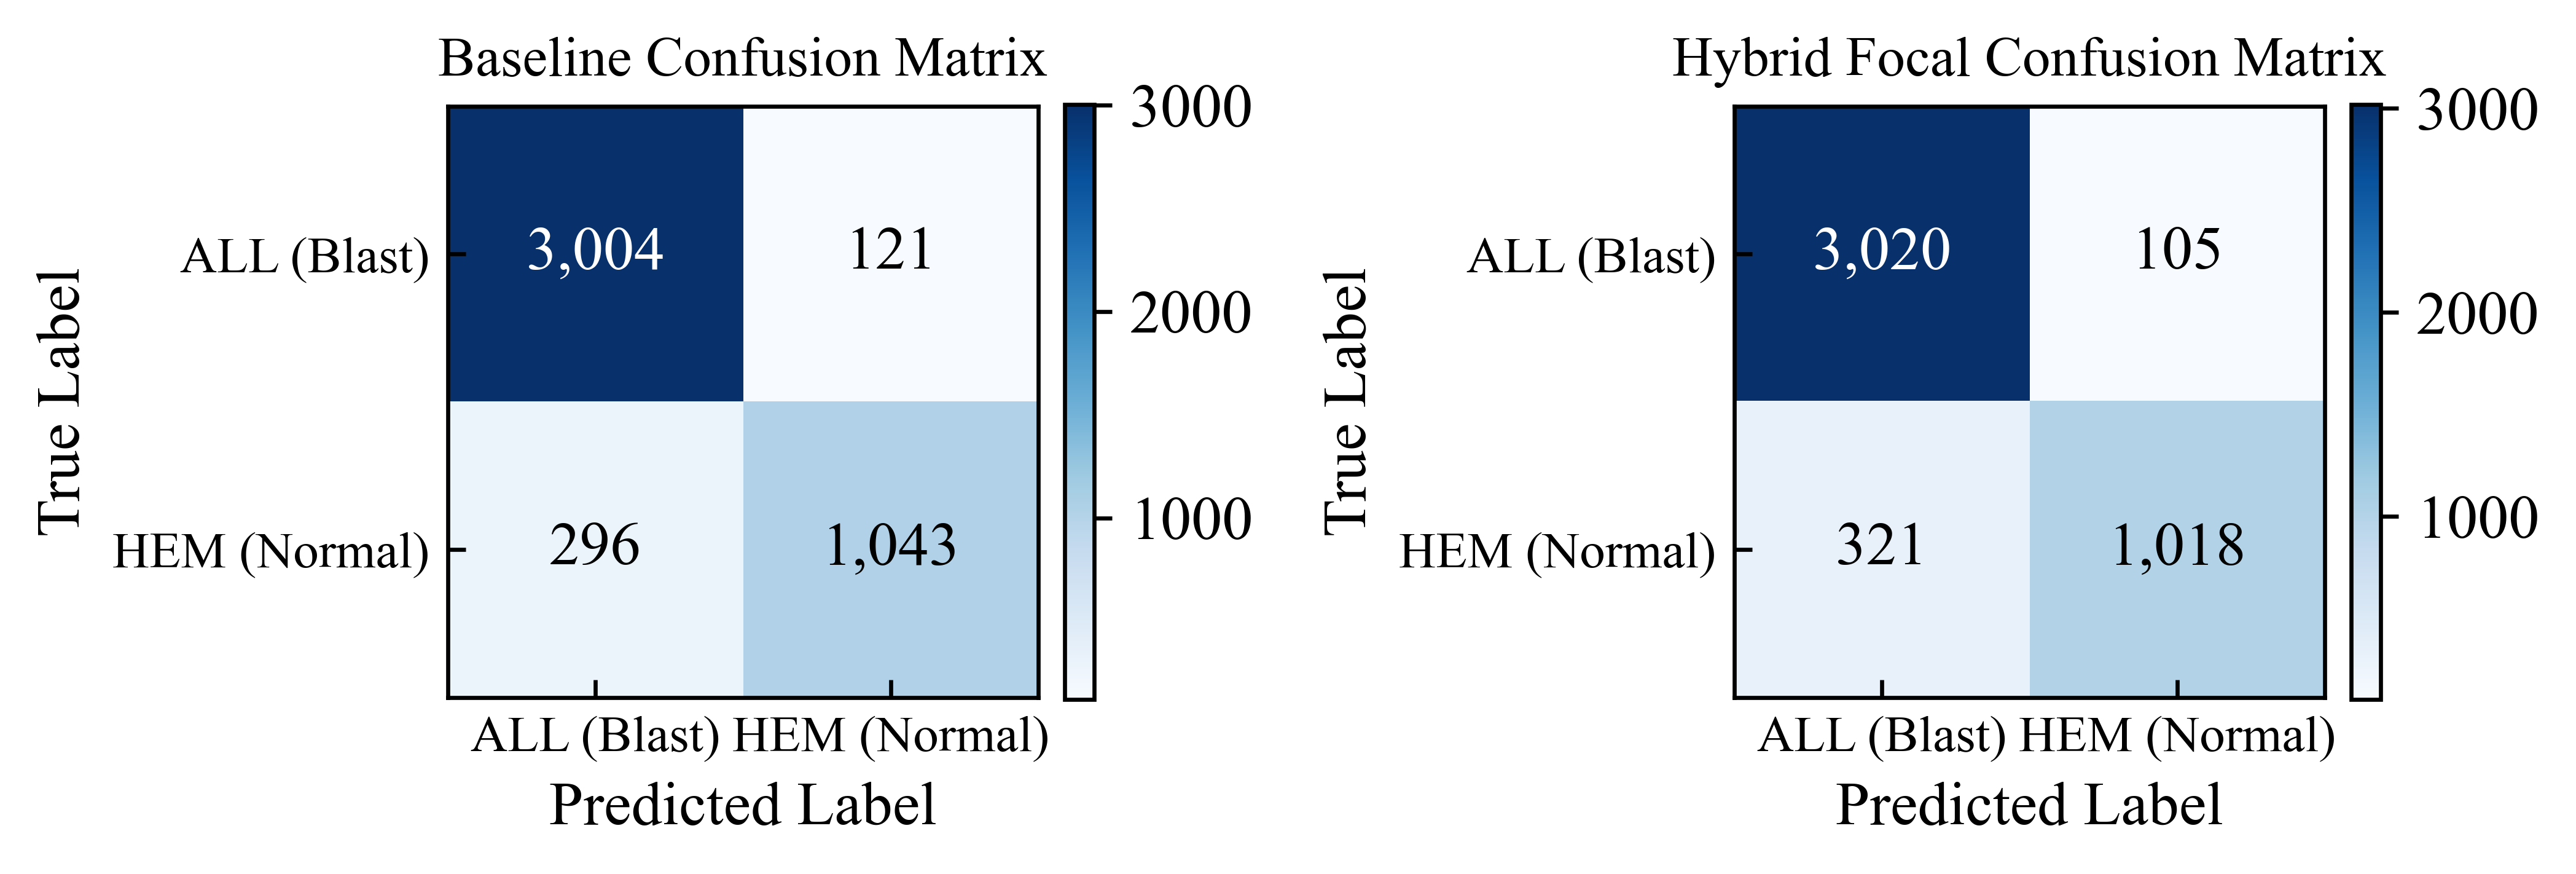
\includegraphics[width=\columnwidth]{figures/comparison_confusion_matrices.png}}
\caption{Side-by-side confusion matrices verifying the targeted reduction in false-negative manifestations provided by hybrid focal learning strategies against standard baselines.}
\label{fig:cm}
\end{figure}

The principal limitation observed within this study pipeline remains the stark computational dependency of the advanced SAM segmentation layer. As structured, SAM constitutes an insurmountable bottleneck for localized processing capabilities on base ARM architectures, forcing its abstraction as a secondary or auxiliary GPU-dependent process. Future translational efforts must endeavor to quantize and extract localized ViT sub-networks specialized uniformly for microscopic boundaries, alongside expansions mapping multi-institutional dataset variants beyond the internal C-NMC cohort scope.

\section{Conclusion}
This paper presents a fully deployable, edge-native technical architecture enabling automated leukemia screening in decentralized clinic environments. Through the systemic integration of hybrid morphological segmentation routines and the progressive unfreezing of deeply compressed CNN parameters, the study solidifies an end-to-end pipeline capable of identifying acute cellular malignancies independent of cloud infrastructure. By enforcing strict subject-disjoint evaluation bounds and prioritizing clinically actionable sensitivity via localized focal operators, the resultant framework deliberately sidesteps brittle mathematical accuracy in favor of deployable geometric viability. Operating effectively under 50\,ms of isolated classifier latency upon Raspberry Pi configurations, this study establishes a robust technological scaffolding for accessible, assistive point-of-care diagnostics within resource-constrained medical landscapes.

\section*{Acknowledgment}
    The authors would like to thank the Cancer Imaging Archive (TCIA) for providing the C-NMC 2019 dataset and the organizers of the ISBI 2019 challenge.

    \begin{thebibliography}{00}
    \bibitem{b1} A. Esteva, K. Chou, S. Yeung, et al., ``Deep learning-enabled medical computer vision,'' \emph{npj Digital Medicine}, vol. 4, no. 1, p. 5, 2021.
    \bibitem{b2} G. Litjens, T. Kooi, B. E. Bejnordi, et al., ``A survey on deep learning in medical image analysis,'' \emph{Medical Image Analysis}, vol. 42, pp. 60-88, 2017.
    \bibitem{b3} S. Shafique and S. Tehsin, ``Acute Lymphoblastic Leukemia Detection and Classification of Its Subtypes Using Pretrained Deep Convolutional Neural Networks,'' \emph{Technology in Cancer Research \& Treatment}, vol. 17, 2018.
    \bibitem{b4} C. Thanh, T. Vun, and N. M. N. A. Hamid, ``Leukemia Blood Cell Image Classification Using Convolutional Neural Network,'' \emph{Procedia Computer Science}, vol. 135, pp. 54-62, 2018.
    \bibitem{b6} H. Guan and M. Liu, ``Domain Adaptation for Medical Image Analysis: A Survey,'' \emph{IEEE Transactions on Biomedical Engineering}, vol. 69, no. 3, pp. 1173--1185, 2022.
    \bibitem{b7} K. K. Mohammed, A. E. Hassanien, and H. M. Afify, ``Refinement of ensemble strategy for acute lymphoblastic leukemia microscopic images using hybrid CNN-GRU-BiLSTM and MSVM classifier,'' \emph{Neural Computing and Applications}, vol. 35, pp. 17415--17427, 2023.
    \bibitem{b8} R. D. Labati, V. Piuri, and F. Scotti, ``Deep learning for acute lymphoblastic leukemia detection,'' \emph{arXiv preprint arXiv:1909.11866}, 2019.
    \bibitem{b9} M. J. Garcia, et al., ``Deep learning assists in acute leukemia detection and cell classification via flow cytometry,'' \emph{Scientific Reports}, vol. 14, p. 58580, 2024.
    \bibitem{b10} S. Rajaraman, et al., ``Leukemia detection and classification using falcon optimization and deep learning,'' \emph{Scientific Reports}, vol. 14, p. 72900, 2024.
    \bibitem{b12} M. Tan and Q. V. Le, ``EfficientNet: Rethinking Model Scaling for Convolutional Neural Networks,'' \emph{arXiv preprint arXiv:1905.11946}, 2019.
    \bibitem{b5} A. Gupta and R. Gupta, ``ALL Challenge dataset of ISBI 2019,'' \emph{The Cancer Imaging Archive}, 2019.

    \bibitem{b_focal}
    T.-Y. Lin, P. Goyal, R. Girshick, K. He, and P. Dollár,
    ``Focal Loss for Dense Object Detection,''
    \textit{IEEE Trans. Pattern Anal. Mach. Intell.},
    vol. 42, no. 2, pp. 318--327, 2020.

    \bibitem{b_jacob2018}
    B. Jacob, S. Kligys, B. Chen, M. Zhu, M. Tang, A. Howard,
    H. Adam, and D. Kalenichenko,
    ``Quantization and Training of Neural Networks for Efficient
    Integer-Arithmetic-Only Inference,''
    in \textit{Proc. IEEE/CVF CVPR}, 2018, pp. 2704--2713.
    \end{thebibliography}

    \end{document}
